\documentclass{beamer}
\usetheme{Singapore}
%\setbeamercolor{structure}{fg=red}
\usepackage{upgreek}
\usepackage{color}
%\def\magyarOptions{hyphenation=huhyphn}
%\usepackage{ae,aecompl}
%\usepackage[T1]{fontenc}
\usepackage[utf8]{inputenc}
%\usepackage[hungarian]{babel}
\usepackage{gensymb}
\usepackage{pgfplots}
\usepackage{pst-plot}
\usepackage{tikz}
\usepgfplotslibrary{external}
\tikzexternalize
\usepackage[version=3]{mhchem}

\normalfont
\title{Felületi szigetelőrétegek ellenállástérképezése fémeken}
\subtitle{Fiatal Analitikusok XXVI. Előadóülése}
\author
{Kiss András, Kiss László\\
\hfill \\
}
\institute
{
  %\inst{1}%
  Általános és Fizikai Kémia Tanszék\\
  Pécsi Tudományegyetem\\
  \hfill \\

  
\includegraphics[width=0.14\textwidth]{pte_logo.eps}\\
  Budapest, 2018. november 12.
}

\date[]

\begin{document}
\frame{\titlepage}  


\begin{frame}
	\centering
	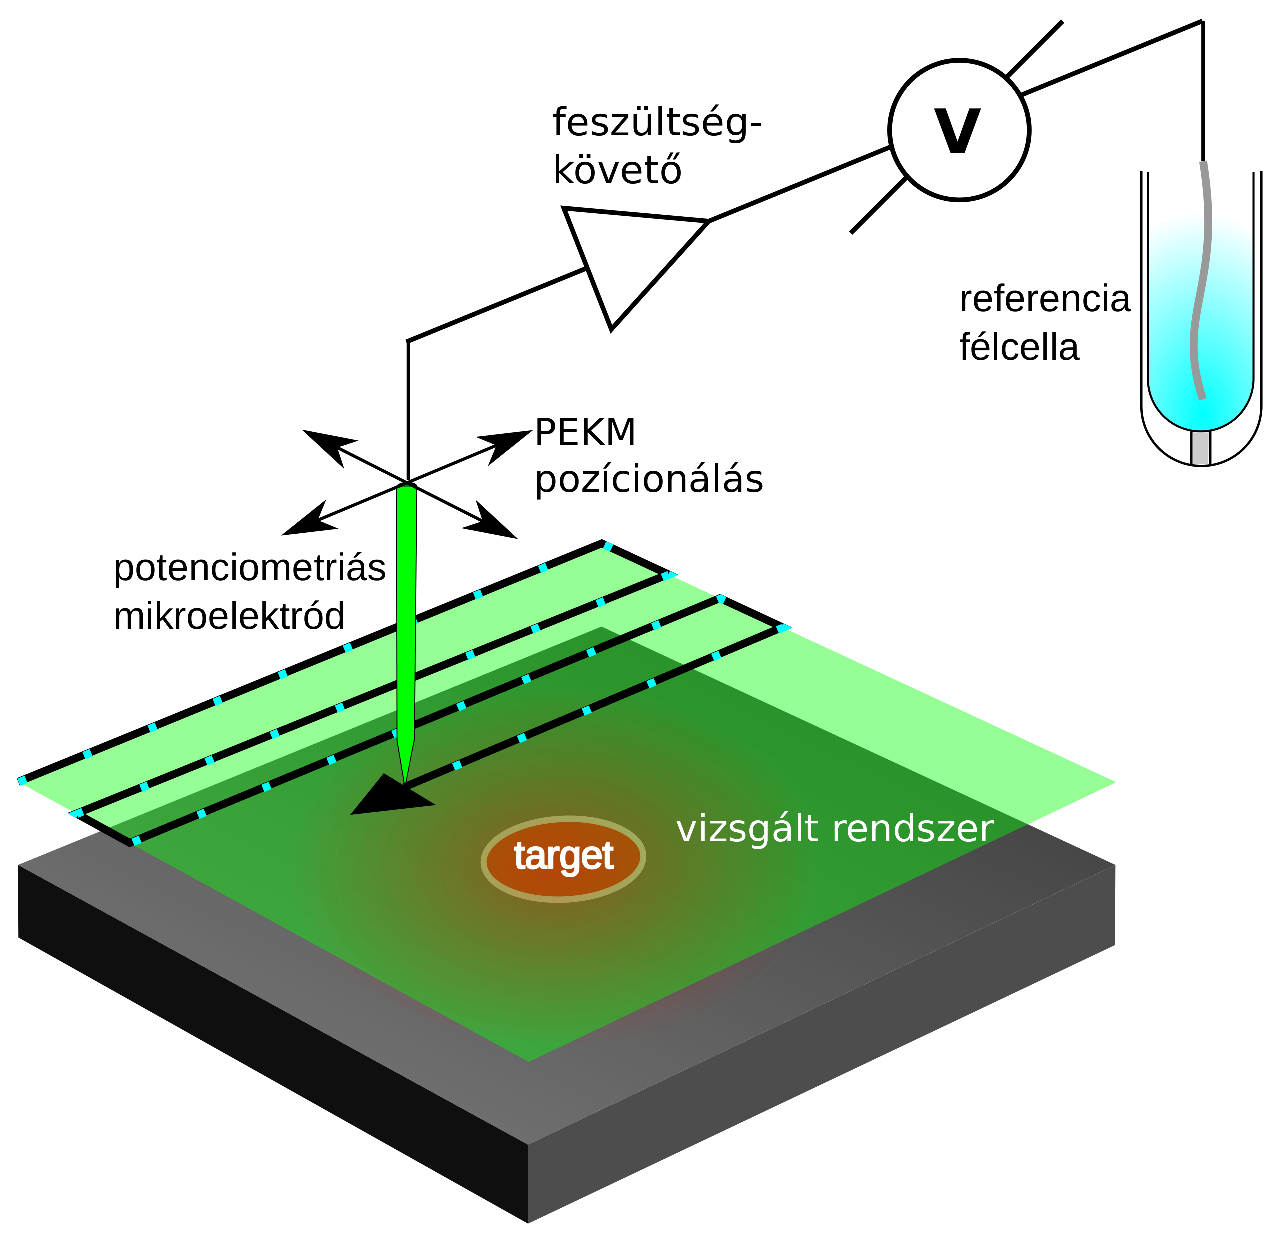
\includegraphics[width=0.6\textwidth]{secm.eps}
	\frametitle{Potenciometriás \underline{p}ásztázó \underline{e}lektro\underline{k}émiai \underline{m}ikroszkóp}
\end{frame}

\begin{frame}
\frametitle{Ion-szelektív mikropipetta}
\framesubtitle{PEKM mérőcsúcs}
\begin{columns}[T] % align columns
\begin{column}{.48\textwidth}

\centering
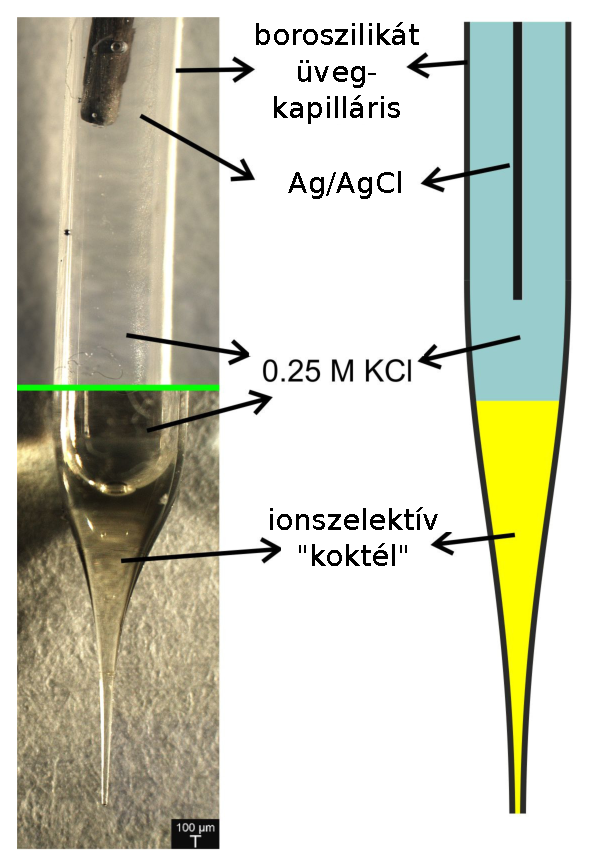
\includegraphics[width=0.9\textwidth]{liquid.eps}
\end{column}%
\hfill%
\begin{column}{.48\textwidth}
%\color{blue}\rule{\linewidth}{4pt}
\centering

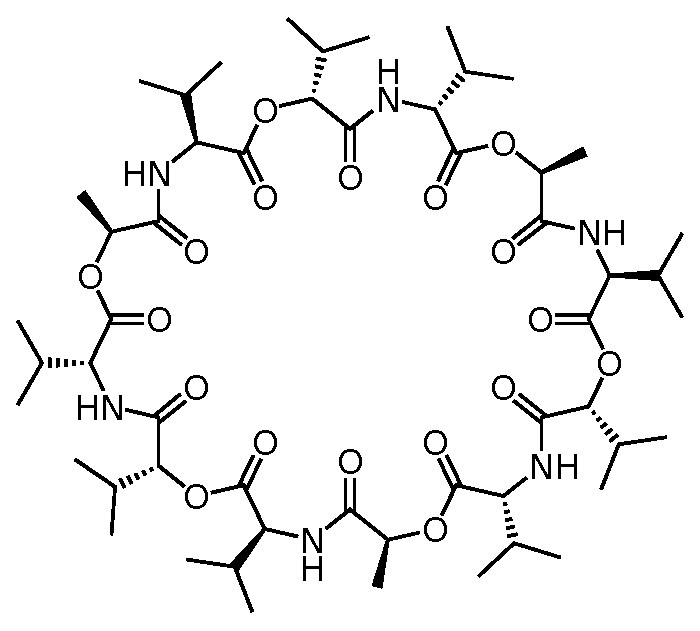
\includegraphics[width=0.8\textwidth]{Valinomycin.eps}

Valinomicin
\vfill

\footnotesize
\begin{equation*}
        E=E^\theta + \frac{RT}{z_iF} \ln \left [ a_i + \sum_{j} \left ( k_{ij}a_j^{z_i/z_j} \right ) \right ]
        \end{equation*}
\normalsize
Nikolszkij--egyenlet
\end{column}%
\end{columns}
\end{frame}

\begin{frame}
	\centering
	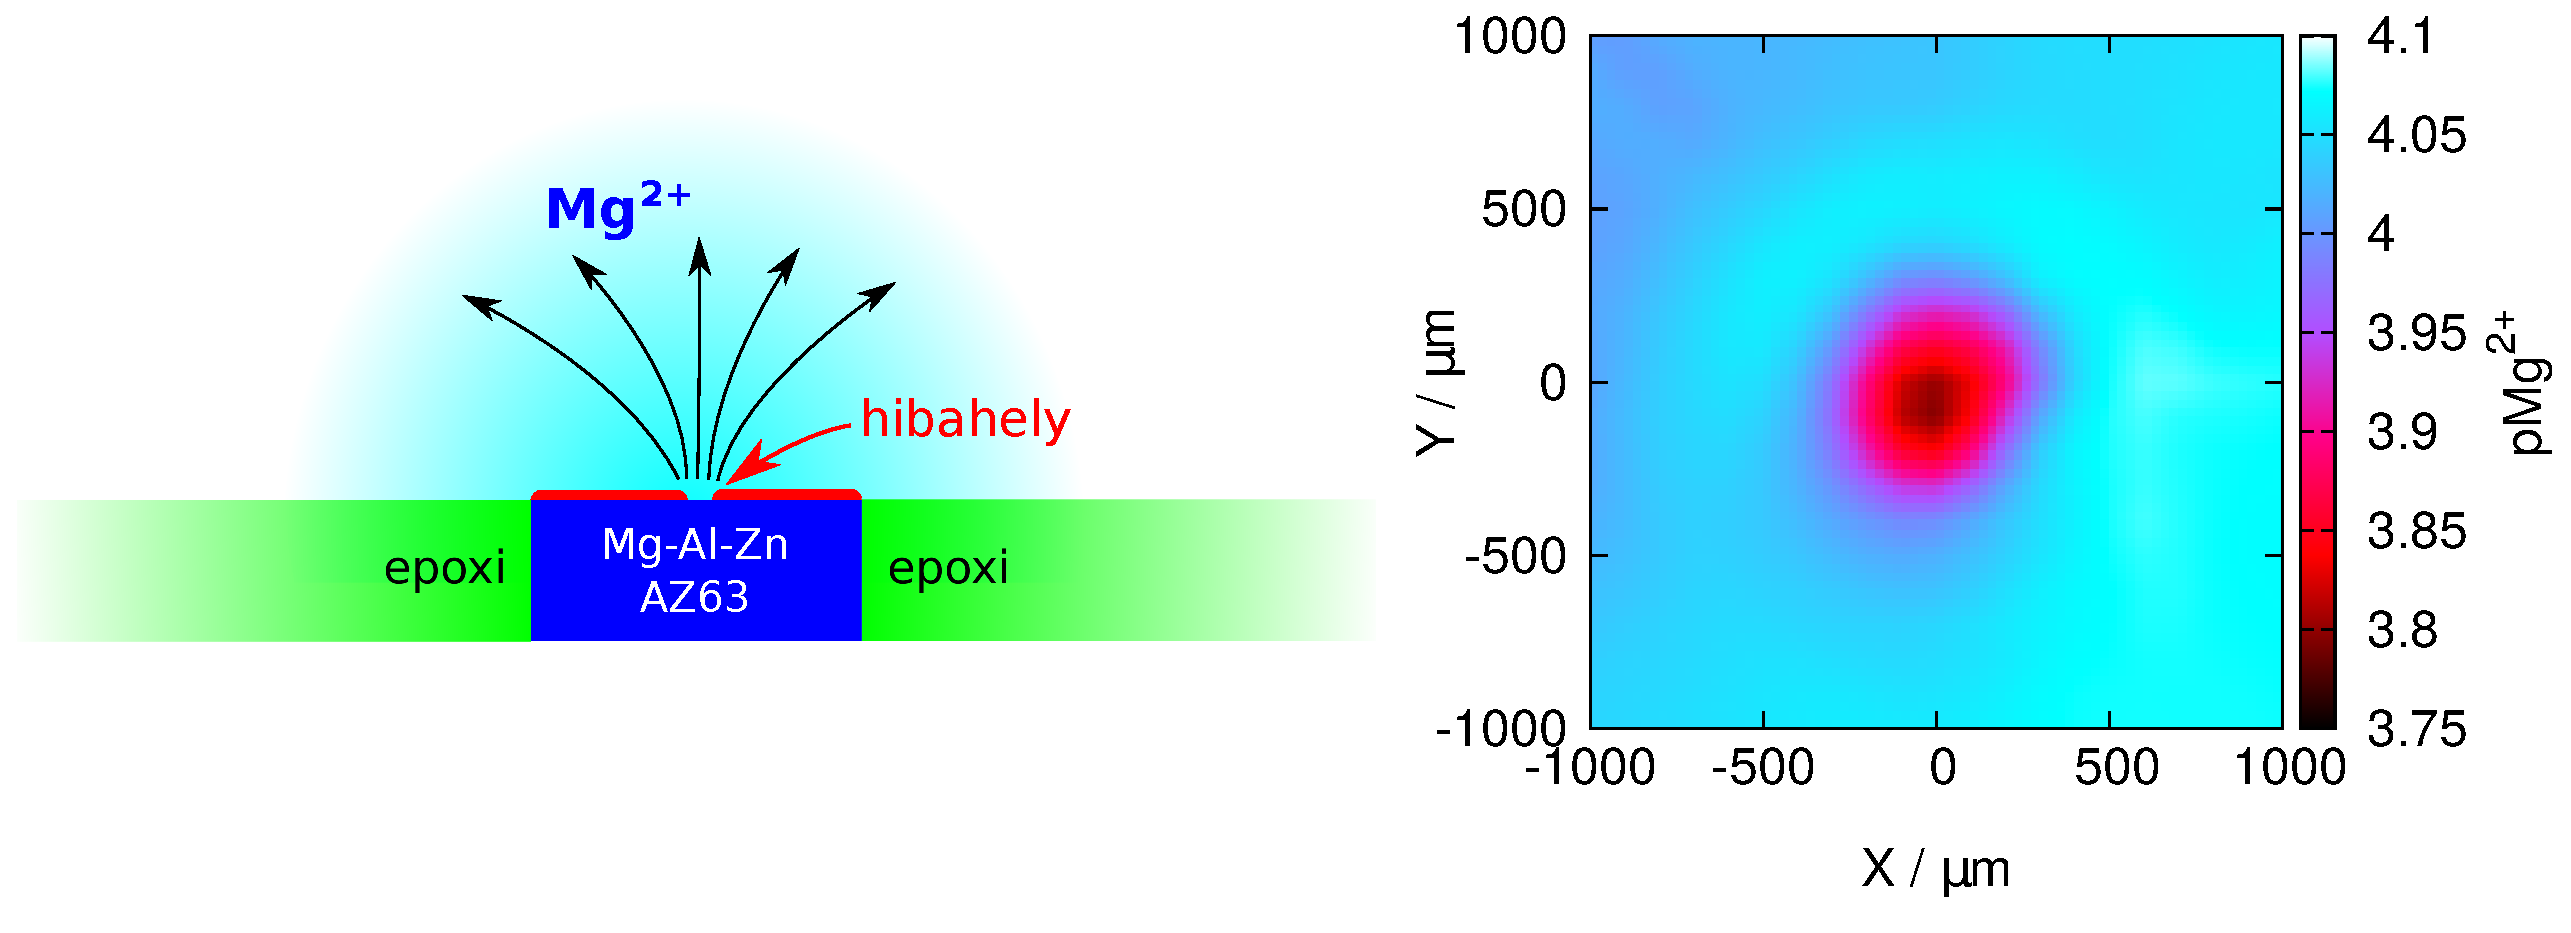
\includegraphics[width=0.9\textwidth]{hiba.eps}
	\frametitle{Korrózióellenes védőbevonat vizsgálata}
	\framesubtitle{Ion-szelektív mikroelektróddal}
\end{frame}

\begin{frame}
	\centering
	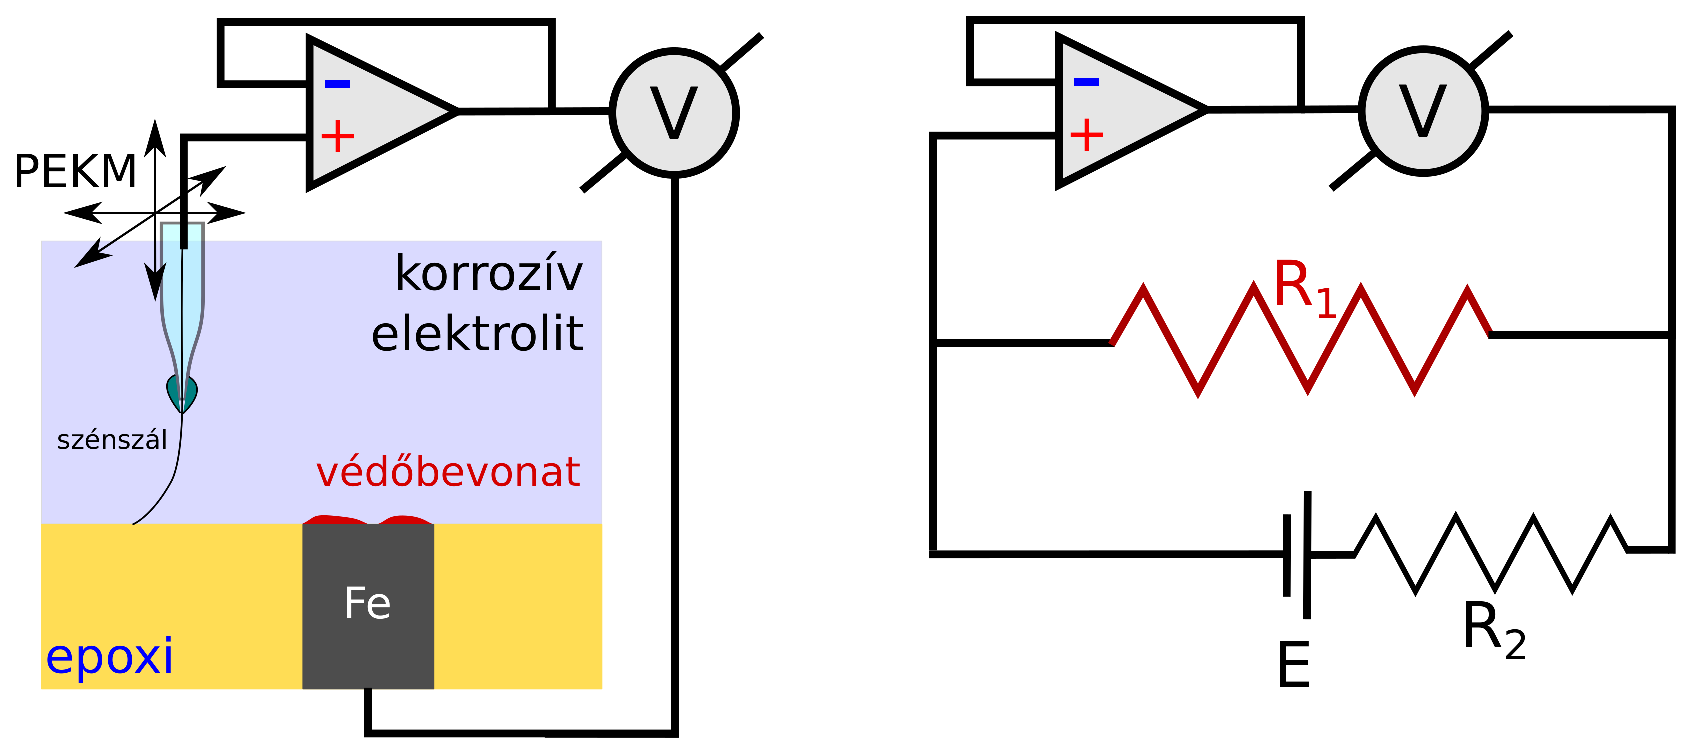
\includegraphics[width=0.9\textwidth]{whisker.eps}
	\frametitle{Direkt kontaktusú pásztázás szénszállal}
%	\framesubtitle{Ionszelektív mikroelektróddal}
\end{frame}

\begin{frame}
\frametitle{Pásztázás polipirrol (1) és polifenol (2) réteggel bevont vas felületen}
\begin{figure}
\centering
% trim = top left bottom right
\includegraphics[trim = 15mm 30mm 0mm 15mm, clip, width=0.3\textwidth, angle=-90]{18012501_deconvoluted.eps}\hspace{0.6cm}\includegraphics[trim = 15mm 30mm 0mm 15mm, clip, width=0.3\textwidth, angle=-90]{18012406_deconvoluted.eps}
%\includegraphics[trim = 350mm 300mm 460mm 250mm, clip, width=0.5\textwidth]{img.jpg}
% trim = left bottom right top
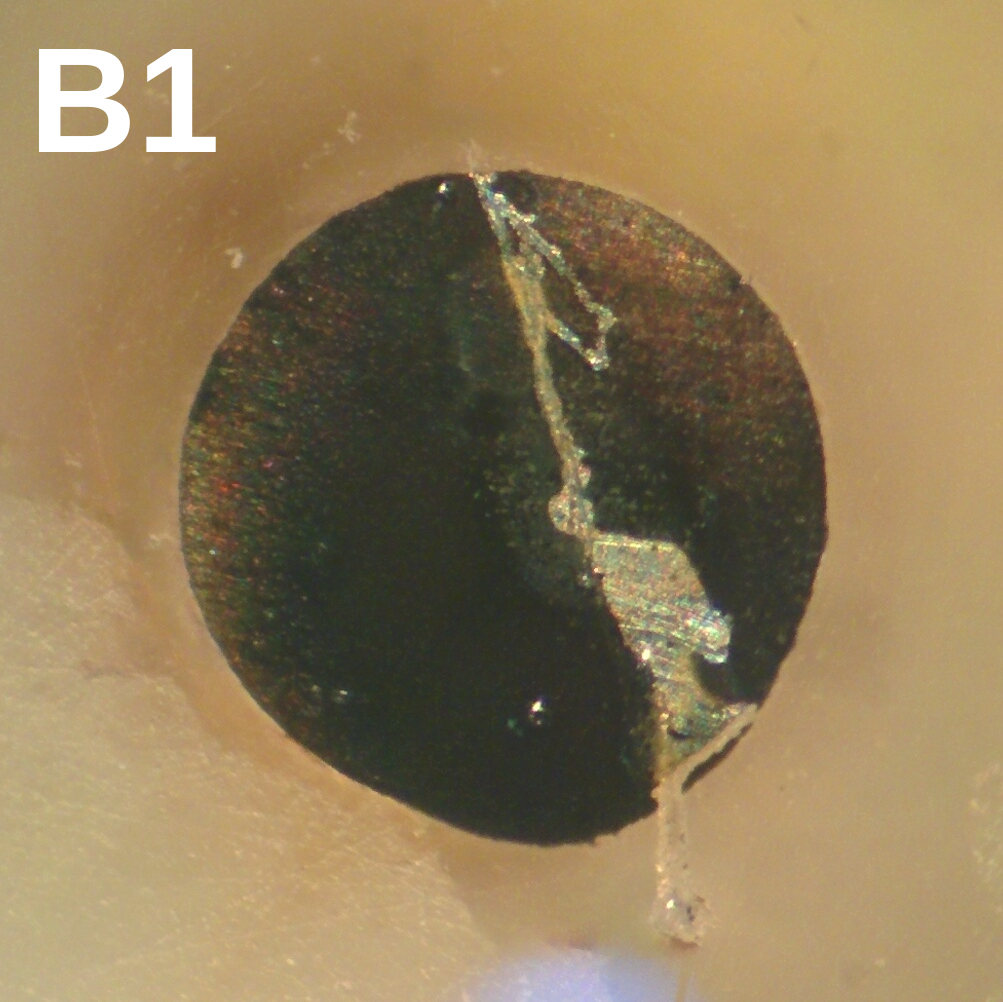
\includegraphics[width=0.25\textwidth]{ppyrrole_cut.jpg}\hspace{2cm}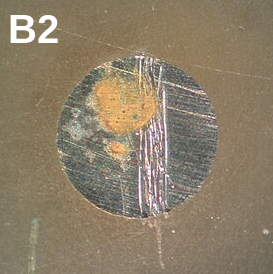
\includegraphics[width=0.25\textwidth]{pphenol_cut.jpg}
\end{figure}
\end{frame}

\begin{frame}
	\centering
	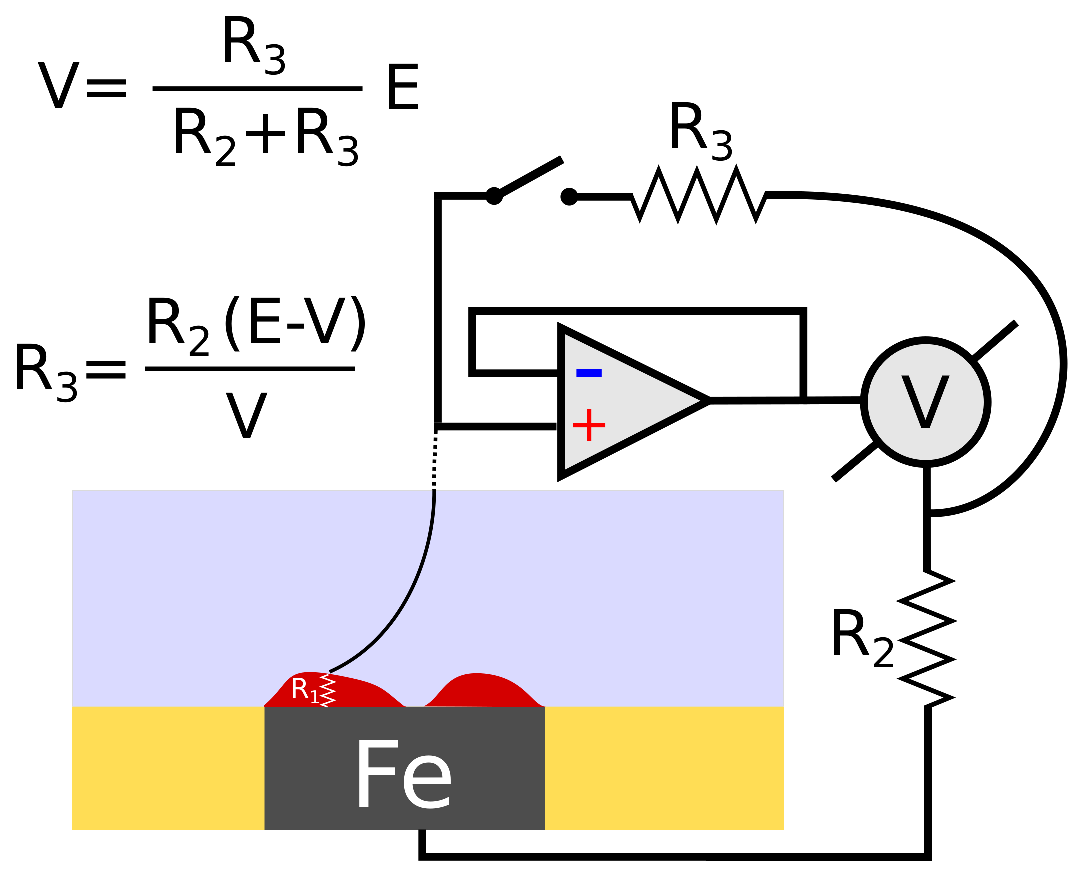
\includegraphics[width=0.7\textwidth]{whisker2.eps}
	\frametitle{Potenciometriás cella ellenállásának (R$_2$) mérése}
	
%	\framesubtitle{Ionszelektív mikroelektróddal}
\end{frame}

\begin{frame}
\frametitle{Polipirrol (1) és polifenol (2) réteggel bevont vas felület ellenállástérképe}
\begin{figure}
\centering
% trim = top left bottom right
\includegraphics[trim = 15mm 30mm 0mm 15mm, clip, width=0.3\textwidth, angle=-90]{18012501_deconvoluted_r.eps}\hspace{0.6cm}\includegraphics[trim = 15mm 30mm 0mm 15mm, clip, width=0.3\textwidth, angle=-90]{18012406_deconvoluted_r.eps}
%\includegraphics[trim = 350mm 300mm 460mm 250mm, clip, width=0.5\textwidth]{img.jpg}
% trim = left bottom right top
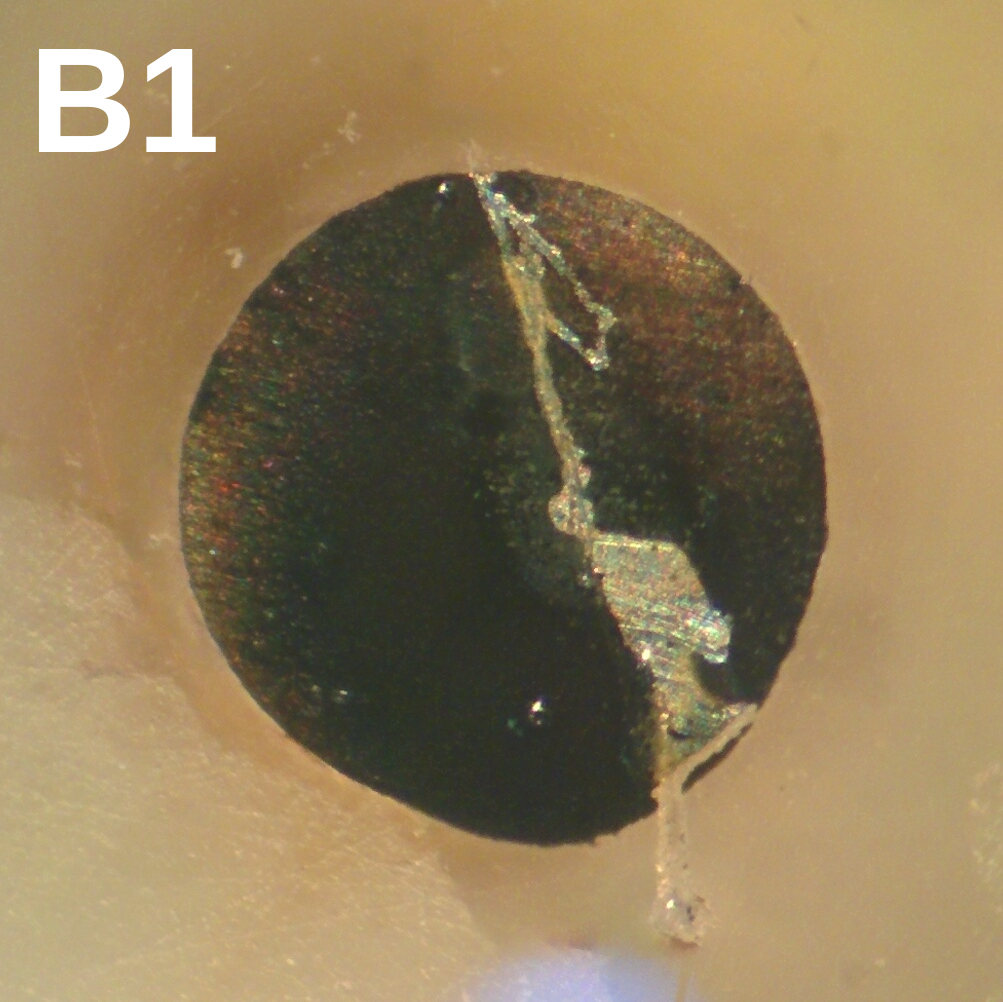
\includegraphics[width=0.25\textwidth]{ppyrrole_cut.jpg}\hspace{2cm}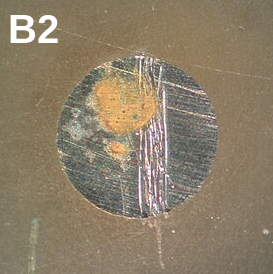
\includegraphics[width=0.25\textwidth]{pphenol_cut.jpg}
\end{figure}
\end{frame}


\begin{frame}
\frametitle{Kezeletlen vas felület ellenállástérképe az idő függvényében}
\framesubtitle{Az oxid-réteg kialakulásának \emph{in situ} nyomonkövetése}
\begin{figure}
\centering
% trim = top left bottom right
\includegraphics[trim = 15mm 30mm 0mm 15mm, clip, width=0.18\textwidth, angle=-90]{17052401_r.eps}
\includegraphics[trim = 15mm 30mm 0mm 15mm, clip, width=0.18\textwidth, angle=-90]{17052402_r.eps}
\includegraphics[trim = 15mm 30mm 0mm 15mm, clip, width=0.18\textwidth, angle=-90]{17052403_r.eps}
\includegraphics[trim = 15mm 30mm 0mm 15mm, clip, width=0.18\textwidth, angle=-90]{17052405_r.eps}
%\includegraphics[trim = 20mm 30mm 0mm 20mm, clip, width=0.3\textwidth, angle=-90]{18011710.eps} 

\vspace{1cm}

% trim = left bottom right top
%\includegraphics[trim = 350mm 300mm 460mm 250mm, clip, width=0.25\textwidth]{IMG.jpg}
%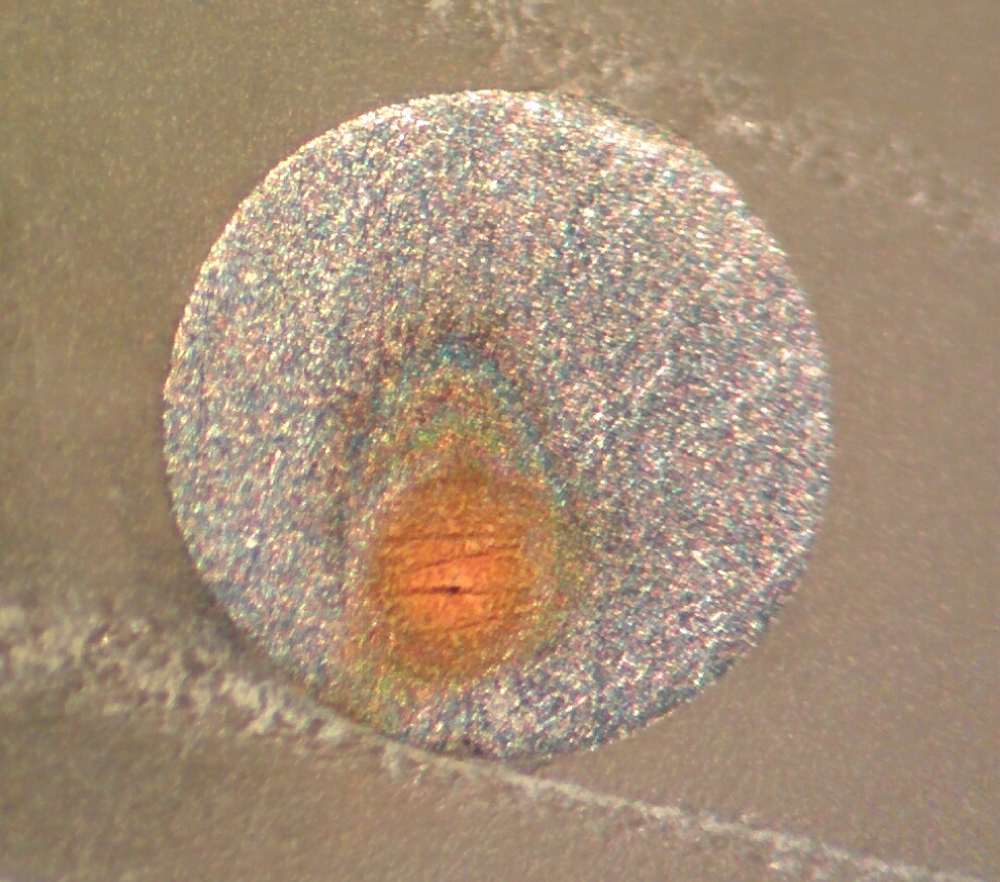
\includegraphics[width=0.3\textwidth]{img1.png}
%\hspace{2cm}
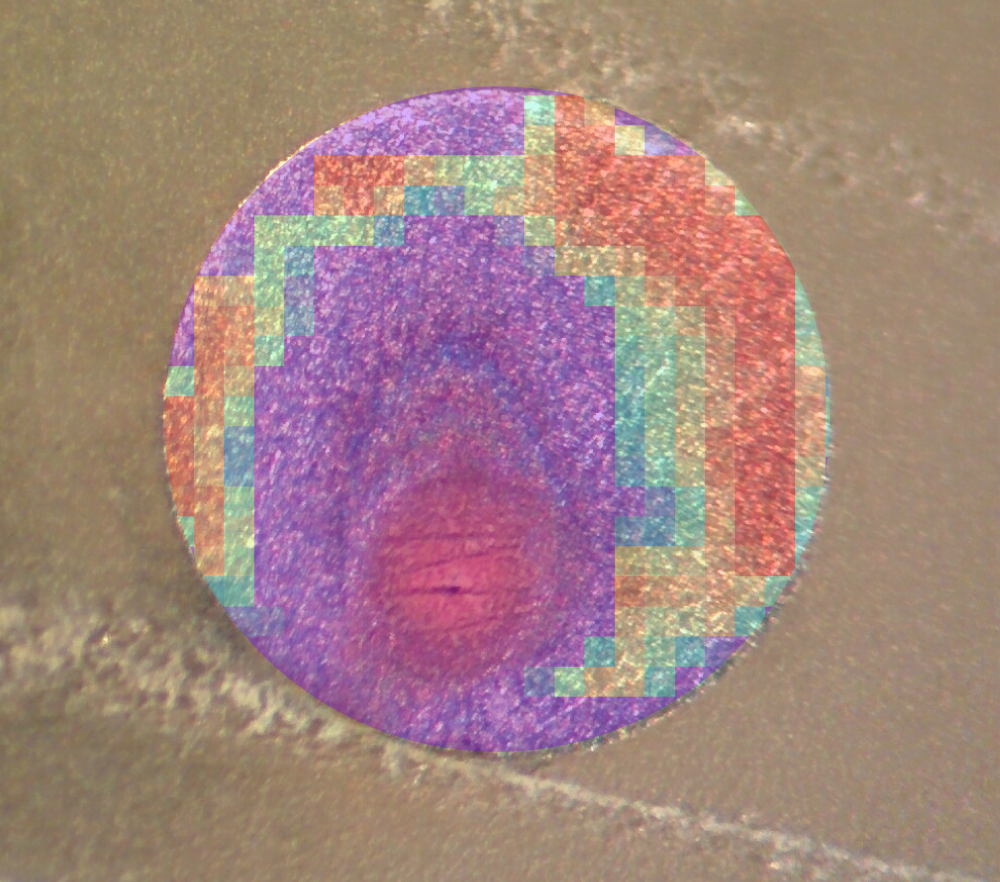
\includegraphics[width=0.3\textwidth]{img2.png}

\end{figure}
\end{frame}


\begin{frame}
	\frametitle{Összefoglalás}
	\centering
\begin{itemize}

\item Vas felületén lévő korrózióellenes bevonatok illetve oxid-réteg ellenállását térképeztem.

\item A technika a potenciometriás pásztázó elektrokémiai mikroszkóppal kivitelezhető, mérőcsúcsként egy egyszerű szénszálat használva.

\item A mért potenciál térképből ellenállás térkép számolható a feszültségosztó elve alapján.

\end{itemize}
\end{frame}

\begin{frame}
	\centering
	Köszönöm a megtisztelő figyelmüket.

%	\includegraphics[width=0.8\textwidth]{thanks.jpg}

\end{frame}



\end{document}
